\documentclass{article}
\usepackage{graphicx}
\graphicspath{ {images/} }
\title{CS 256 Section 2 - Homework 3}
\author{Abhishek Manoj Sharma}
\date{\today}

\begin{document}

\maketitle

\section{Introduction}

The program uses kNN and K-Means clustering algorithm to classify image data. The program is bundled with more than 500 images (landscapes and headshots combined) for this purpose. It extracts image features and classifies an image as landscape or headshot based on the training set. Addtionally, the kNN algorithm is validated using a 3-fold validation set.


\section{kNN Algorithm}
The environment uses Pillow library to apply the "FIND EDGES" filter on an image and then computes the RGB mean and standard deviation of every pixel to build up the training set. Following are the results of view predictions that the agent performed on previously unseen images.
\newline
\newline
\begin{tabular}{ | l | l | l | p{5cm} |}
\hline
File & Expected & Prediction\\ \hline
test1 & Landscape & Landscape \\ \hline
test2 & Landscape & Landscape  \\ \hline
test3 & Landscape & Headshot\\ \hline
test4 & Headshot & Headshot \\ \hline
test5 & Headshot & Landscape\\ \hline
test6 & Landscape & Landscape\\ \hline
test7 & Headshot & Landscape \\ 
\hline
\end{tabular}
\newline
\newline
It is interesting to see that the files test3 and test7 were misclassified as Headshotand Landscape respectively. Following are my observations on this:

\begin{center}
\includegraphics{/test_3.jpg}
\newline
The above image got misclassified as a headshot. In my opinion, the heavy brown shade of the grass and the trees confused the agent to think that this dominant color resembled the skin tone of a person.
\newline
\newline
\includegraphics{/test_7.jpg}
\newline
The above image got misclassified as a landscape. In my opinion, the prominent blues in the background tricked the agent and blues and skies are very dominant across the canvas in landscapes.
\end{center}
\newline
\newline
\newline
\section{3-fold validation}

The 3-fold validation was performed by creating 3 training sets of size 344 each. The 3 validation sets were of the sizes 172 each.
\newline
Interestingly, fold 1 gave the maximum accuracy whereas folds 2 and 3 remained similar to each other. Almost all the folds gave good accuracy near k=5.

{\centering\includegraphics[width=0.8\textwidth]{3_fold_graph.PNG}}
\newline

\section{K-Means Clustering}
Cluster 1 of K-Means Clustering consisted of many headshots, whereas the cluster 2 was dominated by landscapes. On carefully looking at them, I observered that images in cluster 2 are more inclined towards shades of blues and green, whereas the first cluster consists of a lot of dark (especially black shades).

{\centering\includegraphics[width=1\textwidth]{cluster_1.PNG}}

{\centering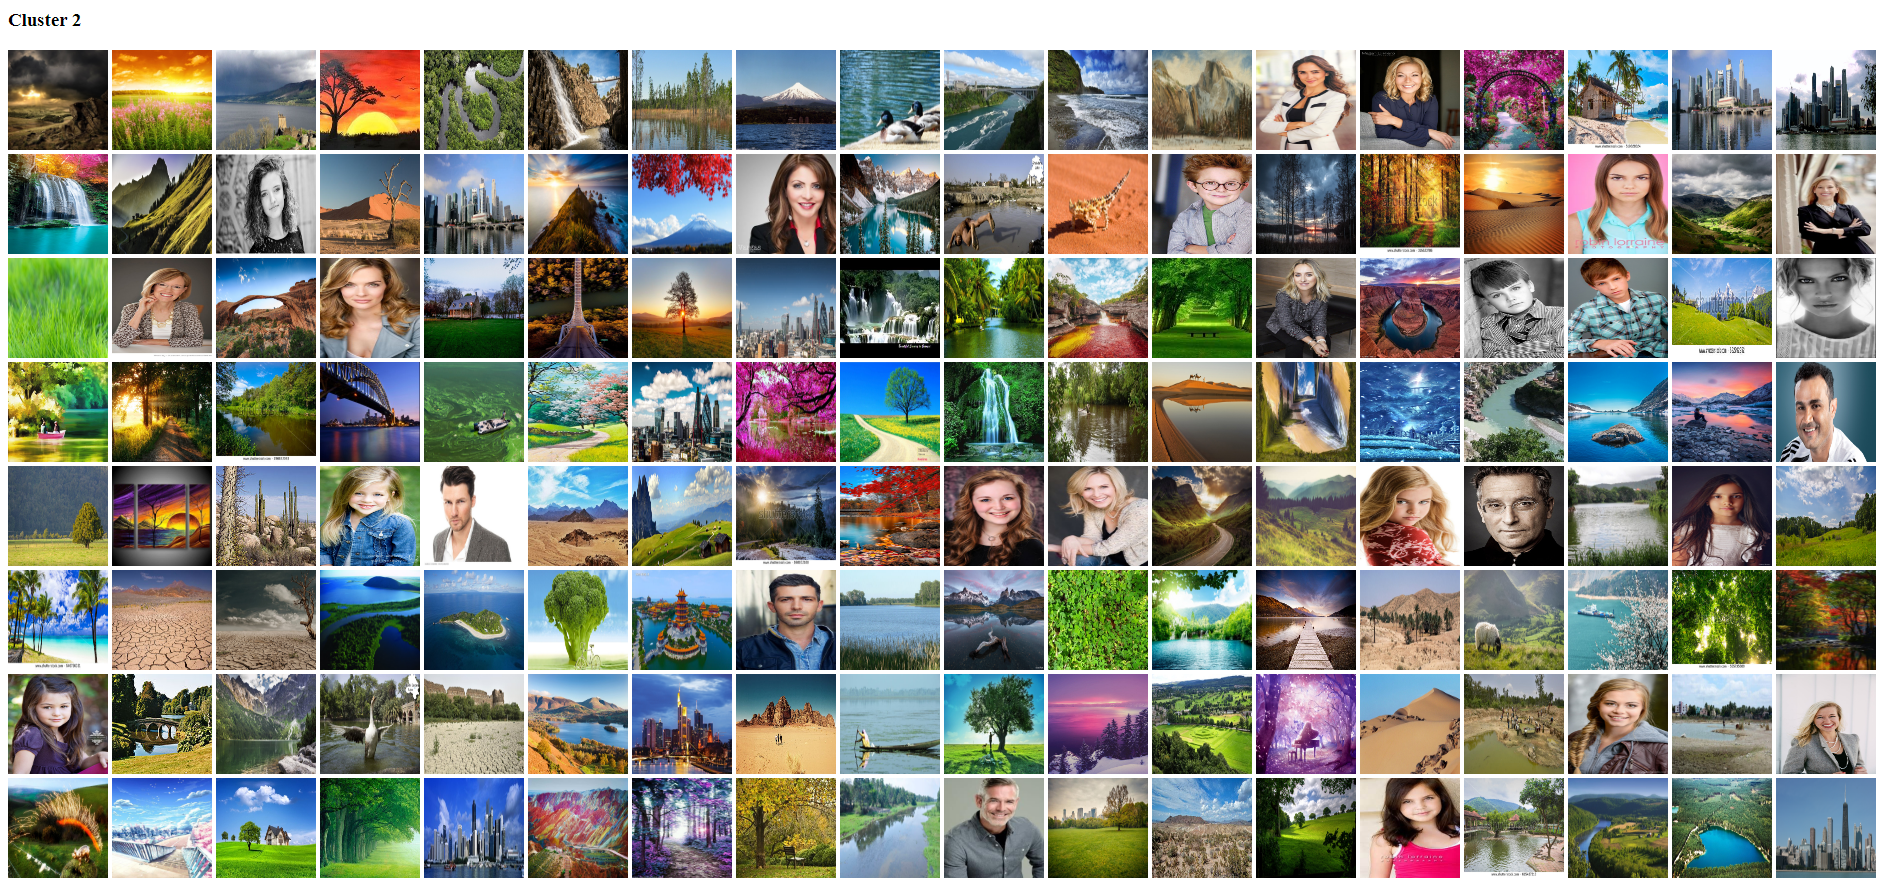
\includegraphics[width=1\textwidth]{cluster_2.PNG}}

\end{document}